\documentclass[14pt]{extbook}
\usepackage{multicol, enumerate, enumitem, hyperref, color, soul, setspace, parskip, fancyhdr} %General Packages
\usepackage{amssymb, amsthm, amsmath, latexsym, units, mathtools} %Math Packages
\everymath{\displaystyle} %All math in Display Style
% Packages with additional options
\usepackage[headsep=0.5cm,headheight=12pt, left=1 in,right= 1 in,top= 1 in,bottom= 1 in]{geometry}
\usepackage[usenames,dvipsnames]{xcolor}
\usepackage{dashrule}  % Package to use the command below to create lines between items
\newcommand{\litem}[1]{\item#1\hspace*{-1cm}\rule{\textwidth}{0.4pt}}
\pagestyle{fancy}
\lhead{Progress Quiz 7}
\chead{}
\rhead{Version B}
\lfoot{3510-5252}
\cfoot{}
\rfoot{Summer C 2021}
\begin{document}

\begin{enumerate}
\litem{
Determine the domain of the function below.\[ f(x) = \frac{4}{20x^{2} +3 x -9} \]\begin{enumerate}[label=\Alph*.]
\item \( \text{All Real numbers.} \)
\item \( \text{All Real numbers except } x = a \text{ and } x = b, \text{ where } a \in [-15, -8] \text{ and } b \in [14, 18] \)
\item \( \text{All Real numbers except } x = a \text{ and } x = b, \text{ where } a \in [-3.75, 0.25] \text{ and } b \in [-0.4, 1.6] \)
\item \( \text{All Real numbers except } x = a, \text{ where } a \in [-3.75, 0.25] \)
\item \( \text{All Real numbers except } x = a, \text{ where } a \in [-15, -8] \)

\end{enumerate} }
\litem{
Choose the graph of the equation below.\[ f(x) = \frac{1}{(x + 2)^2} - 1 \]\begin{enumerate}[label=\Alph*.]
\begin{multicols}{2}\item 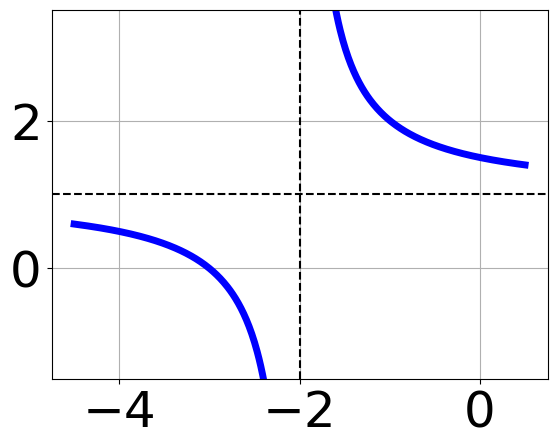
\includegraphics[width = 0.3\textwidth]{../Figures/rationalEquationToGraphAB.png}\item 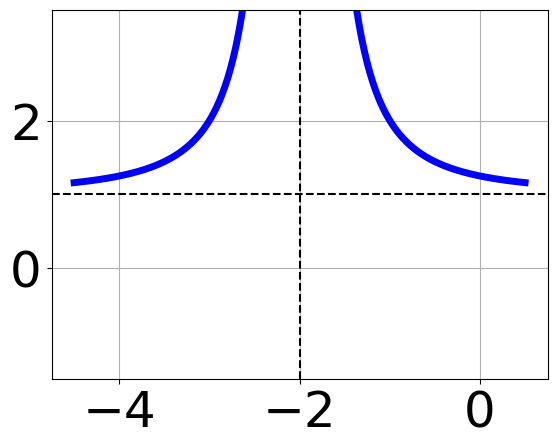
\includegraphics[width = 0.3\textwidth]{../Figures/rationalEquationToGraphBB.png}\item 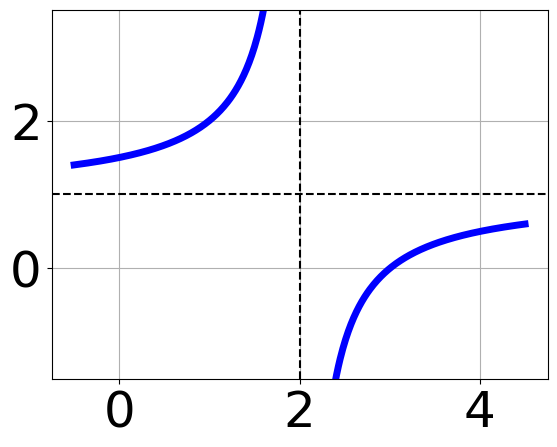
\includegraphics[width = 0.3\textwidth]{../Figures/rationalEquationToGraphCB.png}\item 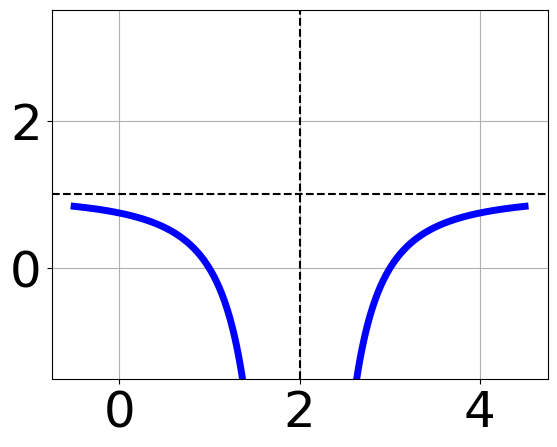
\includegraphics[width = 0.3\textwidth]{../Figures/rationalEquationToGraphDB.png}\end{multicols}\item None of the above.
\end{enumerate} }
\litem{
Choose the graph of the equation below.\[ f(x) = \frac{-1}{(x - 2)^2} - 1 \]\begin{enumerate}[label=\Alph*.]
\begin{multicols}{2}\item 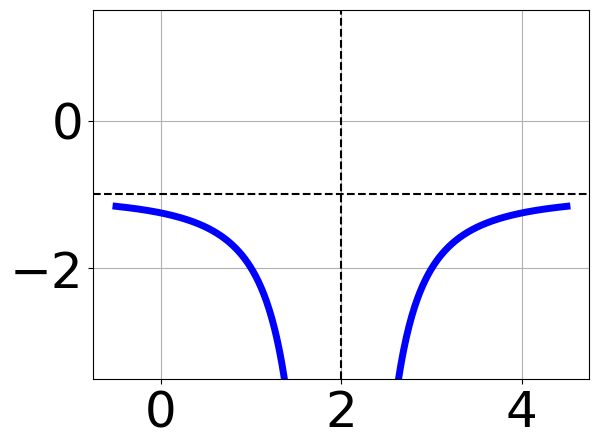
\includegraphics[width = 0.3\textwidth]{../Figures/rationalEquationToGraphCopyAB.png}\item 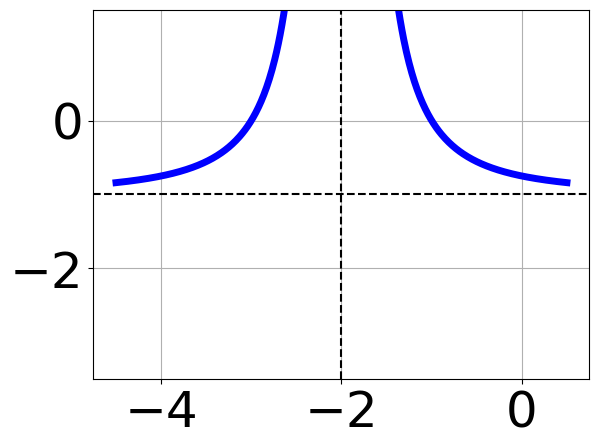
\includegraphics[width = 0.3\textwidth]{../Figures/rationalEquationToGraphCopyBB.png}\item 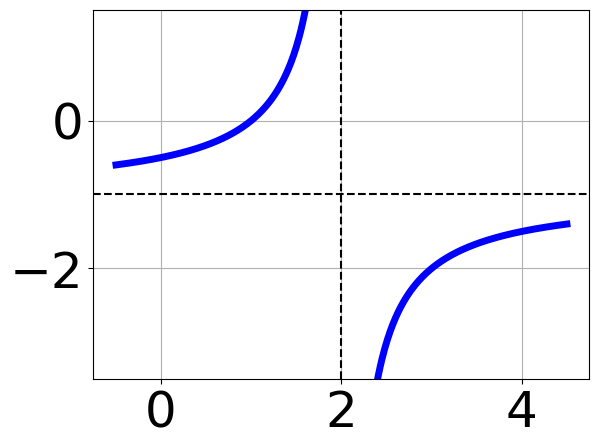
\includegraphics[width = 0.3\textwidth]{../Figures/rationalEquationToGraphCopyCB.png}\item 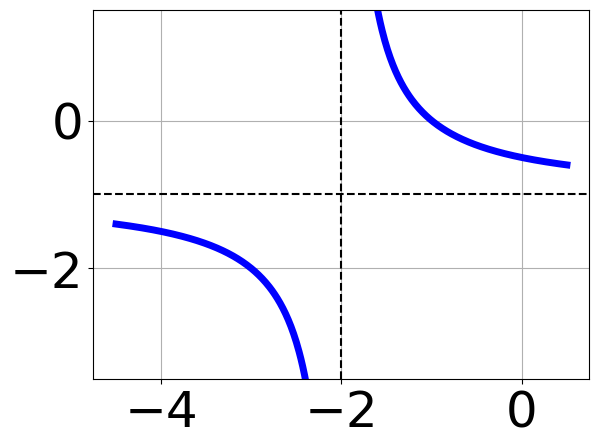
\includegraphics[width = 0.3\textwidth]{../Figures/rationalEquationToGraphCopyDB.png}\end{multicols}\item None of the above.
\end{enumerate} }
\litem{
Choose the equation of the function graphed below.
\begin{center}
    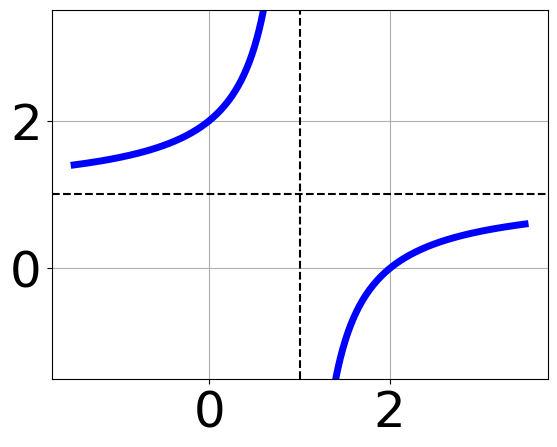
\includegraphics[width=0.5\textwidth]{../Figures/rationalGraphToEquationB.png}
\end{center}
\begin{enumerate}[label=\Alph*.]
\item \( f(x) = \frac{1}{(x - 1)^2} + 2 \)
\item \( f(x) = \frac{-1}{(x + 1)^2} + 2 \)
\item \( f(x) = \frac{-1}{x + 1} + 2 \)
\item \( f(x) = \frac{1}{x - 1} + 2 \)
\item \( \text{None of the above} \)

\end{enumerate} }
\litem{
Choose the equation of the function graphed below.
\begin{center}
    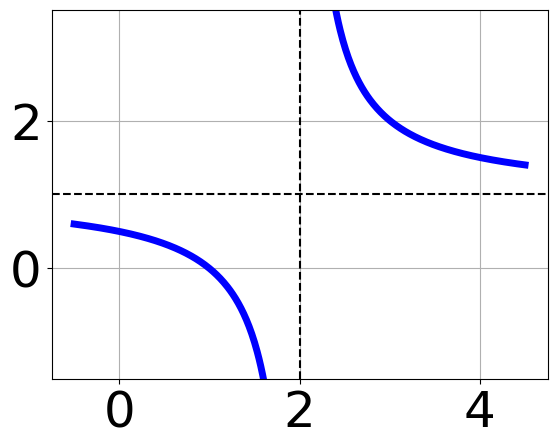
\includegraphics[width=0.5\textwidth]{../Figures/rationalGraphToEquationCopyB.png}
\end{center}
\begin{enumerate}[label=\Alph*.]
\item \( f(x) = \frac{-1}{(x + 2)^2} + 1 \)
\item \( f(x) = \frac{-1}{x + 2} + 1 \)
\item \( f(x) = \frac{1}{(x - 2)^2} + 1 \)
\item \( f(x) = \frac{1}{x - 2} + 1 \)
\item \( \text{None of the above} \)

\end{enumerate} }
\litem{
Solve the rational equation below. Then, choose the interval(s) that the solution(s) belongs to.\[ \frac{5}{5x + 7} + -5 = \frac{3}{10x + 14} \]\begin{enumerate}[label=\Alph*.]
\item \( x_1 \in [-1.27, -1.2] \text{ and } x_2 \in [1.54,2.54] \)
\item \( x_1 \in [-1.37, -1.31] \text{ and } x_2 \in [-2.26,-0.26] \)
\item \( \text{All solutions lead to invalid or complex values in the equation.} \)
\item \( x \in [-1.26,-0.26] \)
\item \( x \in [1.46,1.65] \)

\end{enumerate} }
\litem{
Solve the rational equation below. Then, choose the interval(s) that the solution(s) belongs to.\[ \frac{65}{-117x -39} + 1 = \frac{65}{-117x -39} \]\begin{enumerate}[label=\Alph*.]
\item \( x \in [-0.2,0.5] \)
\item \( \text{All solutions lead to invalid or complex values in the equation.} \)
\item \( x_1 \in [-0.7, -0.1] \text{ and } x_2 \in [-0.2,1.3] \)
\item \( x \in [-2.33,0.67] \)
\item \( x_1 \in [-0.7, -0.1] \text{ and } x_2 \in [-1.4,-0.3] \)

\end{enumerate} }
\litem{
Determine the domain of the function below.\[ f(x) = \frac{5}{15x^{2} +21 x -18} \]\begin{enumerate}[label=\Alph*.]
\item \( \text{All Real numbers except } x = a \text{ and } x = b, \text{ where } a \in [-19, -14] \text{ and } b \in [15, 18] \)
\item \( \text{All Real numbers except } x = a, \text{ where } a \in [-3, -1] \)
\item \( \text{All Real numbers.} \)
\item \( \text{All Real numbers except } x = a \text{ and } x = b, \text{ where } a \in [-3, -1] \text{ and } b \in [-1.4, 2.6] \)
\item \( \text{All Real numbers except } x = a, \text{ where } a \in [-19, -14] \)

\end{enumerate} }
\litem{
Solve the rational equation below. Then, choose the interval(s) that the solution(s) belongs to.\[ \frac{7x}{2x + 7} + \frac{-4x^{2}}{6x^{2} +27 x + 21} = \frac{-6}{3x + 3} \]\begin{enumerate}[label=\Alph*.]
\item \( x_1 \in [-3.55, -2.83] \text{ and } x_2 \in [-2.09,-0.1] \)
\item \( x \in [-1.49,-0.72] \)
\item \( x_1 \in [-2.46, -1.32] \text{ and } x_2 \in [-0.44,3.39] \)
\item \( x \in [-3.55,-2.83] \)
\item \( \text{All solutions lead to invalid or complex values in the equation.} \)

\end{enumerate} }
\litem{
Solve the rational equation below. Then, choose the interval(s) that the solution(s) belongs to.\[ \frac{4x}{6x -2} + \frac{-2x^{2}}{36x^{2} +24 x -12} = \frac{7}{6x + 6} \]\begin{enumerate}[label=\Alph*.]
\item \( x_1 \in [-0.19, 1.3] \text{ and } x_2 \in [-2,0] \)
\item \( \text{All solutions lead to invalid or complex values in the equation.} \)
\item \( x \in [-1.35,-0.38] \)
\item \( x_1 \in [-0.47, 0.19] \text{ and } x_2 \in [0.99,1.99] \)
\item \( x \in [-0.19,1.3] \)

\end{enumerate} }
\end{enumerate}

\end{document}